\documentclass[12pt]{document}

\usepackage[ngerman]{babel}% change this for your language

%thanks david
\setlength{\parindent}{0pt}
\setlength{\parskip}{4pt}

%load any additional packages
\usepackage{amssymb}
% Korrektes Kodieren des in und outputs
\usepackage[T1]{fontenc}
\usepackage[utf8]{inputenc}    % UTF-8
\usepackage{url}

\usepackage{float}

% better tables
\usepackage{tabularx} % in the preamble

% links across the toc
\usepackage[linkcolor=black,colorlinks=true,citecolor=black,filecolor=black]{hyperref}

\usepackage[sorting=none,backend=biber,style=numeric]{biblatex}
% brauche et al. anstatt u. a.
\DefineBibliographyStrings{german}{andothers={et al\adddot}}
\addbibresource{refs.bib}

%shorthand für tiefstellen
\usepackage{subscript}

\usepackage{mathtools}

\usepackage{amsmath}

%input macros (i.e. write your own macros file called mymacros.tex 
%and uncomment the next line)
%\include{mymacros}

\title{Mein Super Maturaarbeit Titel}   %note \\[1ex] is a line break in the title

\author{Mein Name}             %your name
\college{MNG Rämibühl}  %your college

\renewcommand{\submittedtext}{4. Januar 2016}
\renewcommand{\supervisor}{Betreuende Lehrperson: David Sichau}
\degree{Maturitätsarbeit}     %the degree
\degreedate{}         %the degree date


\usepackage{biblatex}


\addbibresource{refs.bib}% In diesem File ist die Bibliographie gespeichert.



%end the preamble and start the document
\begin{document}


\maketitle                  % create a title page from the preamble info
\begin{abstract}
Hier kommt der Abstract.
\end{abstract}       % include the abstract


\begin{romanpages}          % start roman page numbering
\tableofcontents            % generate and include a table of contents
\end{romanpages}            % end roman page numbering

%now include the files of latex for each of the chapters etc
\chapter{Einleitung}

\textit{Umgang mit grammatikalischen Geschlechtern: Aus Gründen der Spracheleganz wird vor allem die männliche Form (zum Beispiel "`Benutzer"') verwendet. Die weibliche Form ist jedoch sinngemäss mitgemeint.}

\section{Blabla}



Hier ein Beispiel für eine Referenz zu einem Buch \cite{viz}. 



So macht man ein Text Zitat \textit{The Eyes Have It: A Task by Data Type for Information Visualizations} von B. Shneiderman \cite{shneiderman}. 


So verweisst man auf eine Abbildung \ref{fig:nytimes-taxes}.

\begin{figure}[H]
	\centering
	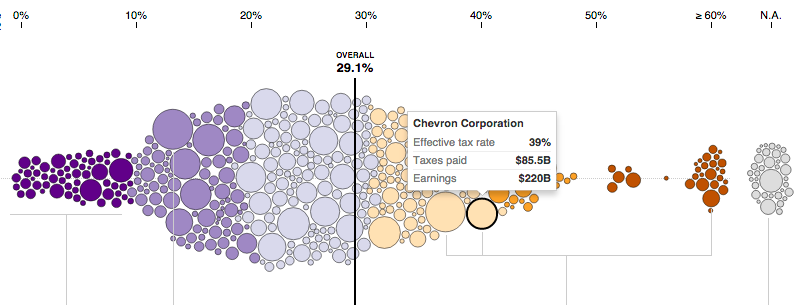
\includegraphics[width=\linewidth]{images/nytimes-taxes-zugeschnitten}
	\caption[Blasendiagramm in The New York Times (\citedate{nytimes-taxes})]{Ein Blasendiagramm, das Steuerabgaben und Steuersätze von US-Firmen darstellt. \cite{nytimes-taxes}}
	\label{fig:nytimes-taxes}% das braucht man um darauf zu verweisen
\end{figure}

\chapter{Hauptteil}

\section{Ein super Titel}
	
\chapter{Schlusswort}

Ein tolles Schlusswort


\newpage
%now enable appendix numbering format and include any appendices
\appendix


\chapter{Literaturverzeichnis}
\printbibliography[heading=none]     %use a bibtex bibliography file refs.bib

\newpage
\chapter{Abbildungsverzeichnis}
\makeatletter
\@starttoc{lof} % Print List of Figures
\makeatother

\newpage
\chapter{Bestätigung der Eigenständigkeit}
Der Unterzeichnete bestätigt mit Unterschrift, dass die Arbeit selbständig verfasst und in schriftliche Form gebracht worden ist, dass sich die Mitwirkung anderer Personen auf Beratung und Korrekturlesen beschränkt hat und dass alle verwendeten Unterlagen und Gewährspersonen aufgeführt sind.
 

\end{document}